\clearpage
\section{Laser}

A SoC (System-on-a-Chip) solution for optical distance measurements applications. The PulsedLight LIDAR has a 4.7 - 5.5 V nominal and 6 V potentially maximum DC operating range. The sensor has a theoretical limit of 40m range and 100Hz rep rate. The laser emitters' accuracy is estimated to be +/- 2.5cm with an aquisition time of less then 0.02sec. These specifications allows us to get an accurate image of the environments specified in our test cases.
%TODO: Specify testing environments in the testsing section.

%How the laser works

\begin{figure}[H]
	\centering
	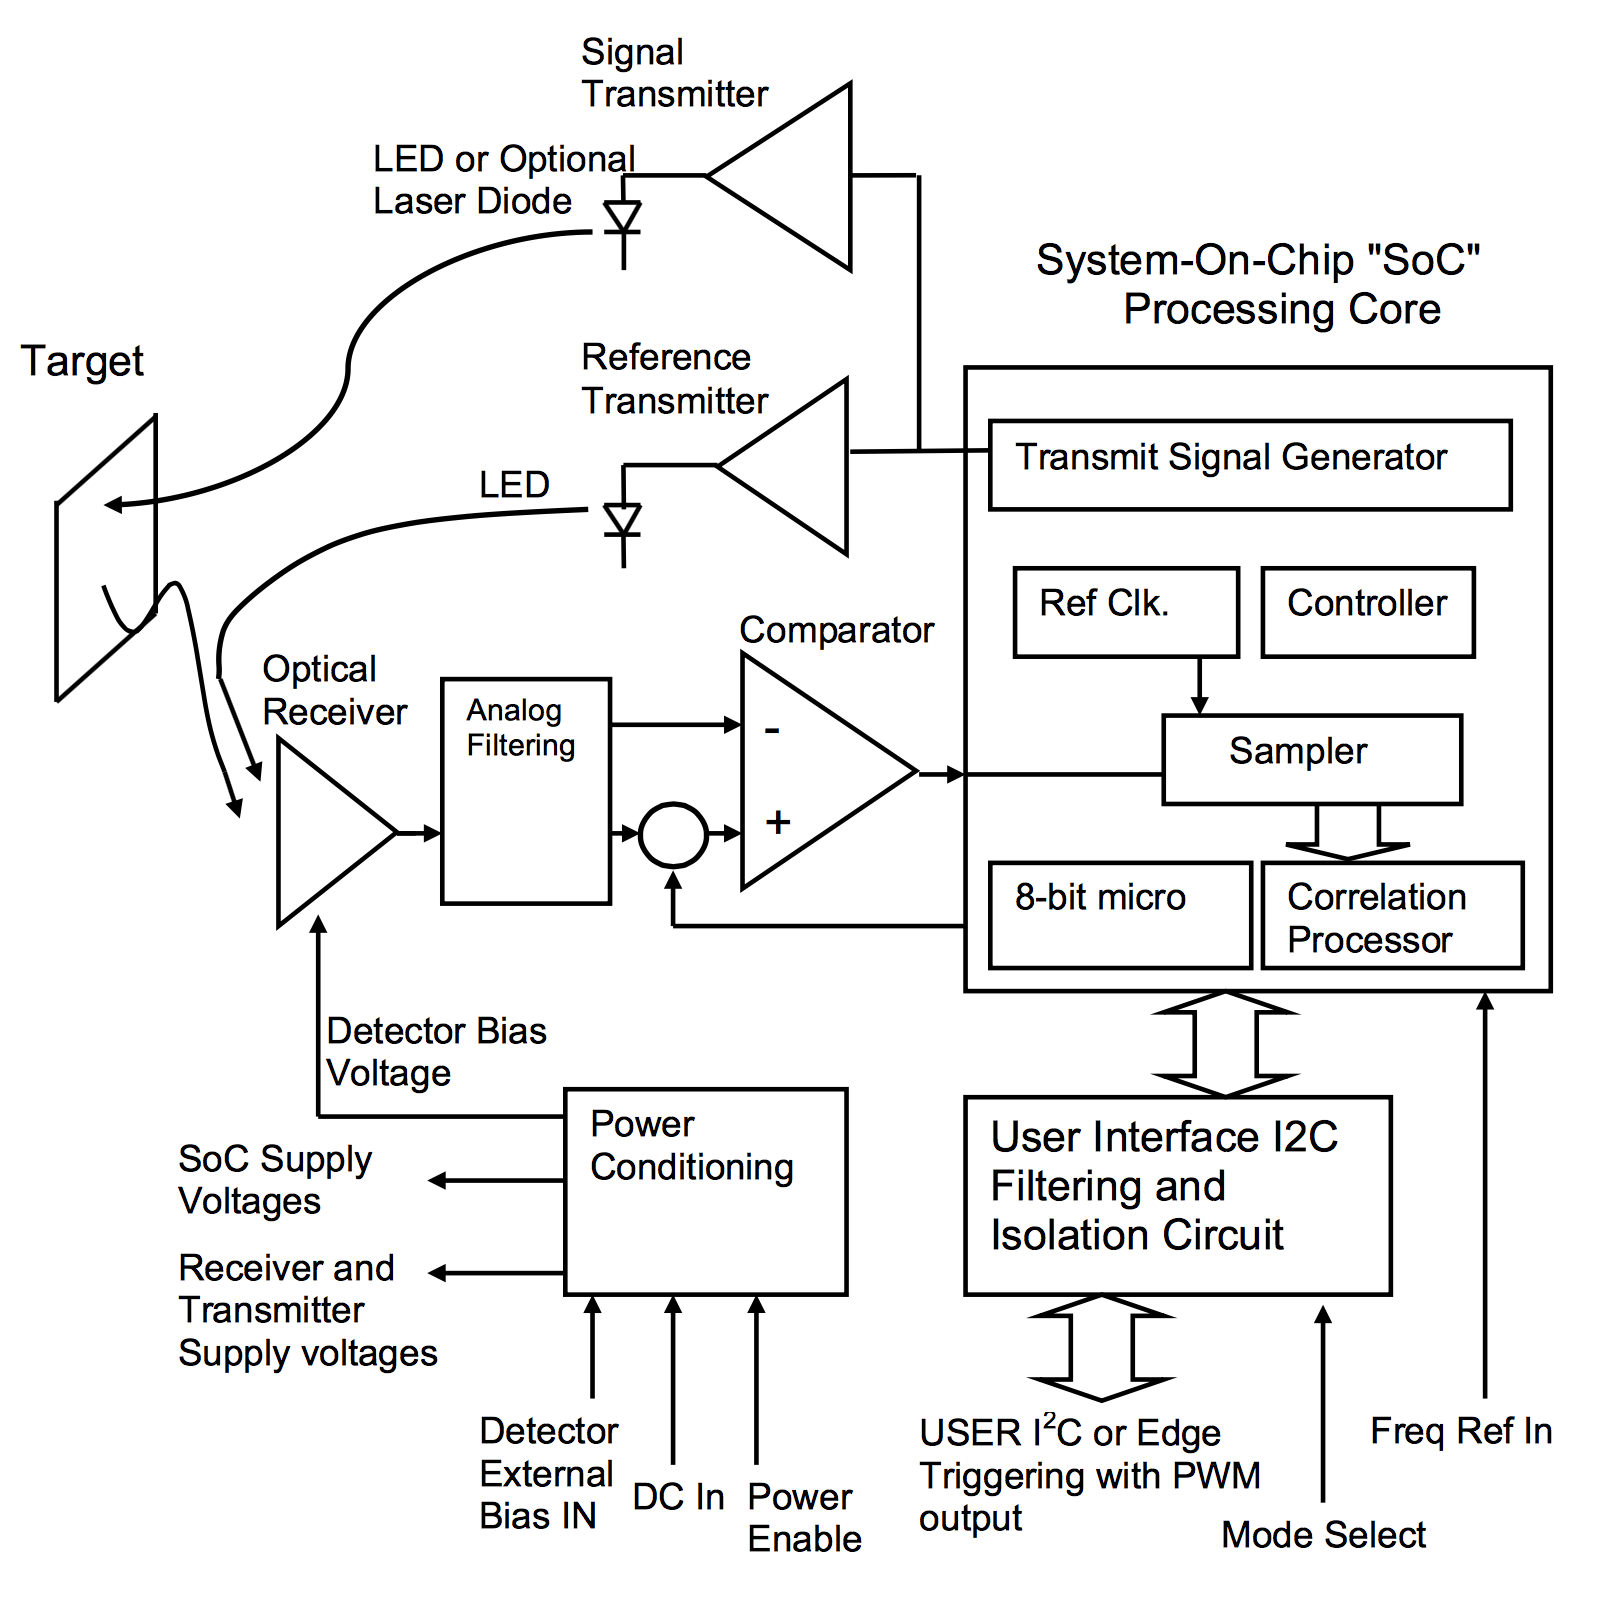
\includegraphics[scale=.4]{images/internallidar.png}
	\caption{The internal of the PulsedLight LIDAR sensor}
	\label{fig:internallidar}
\end{figure}

%diagram showing the laser signal

The assembling of the laser happened in the following way:

\begin{figure}[H]
	\centering
	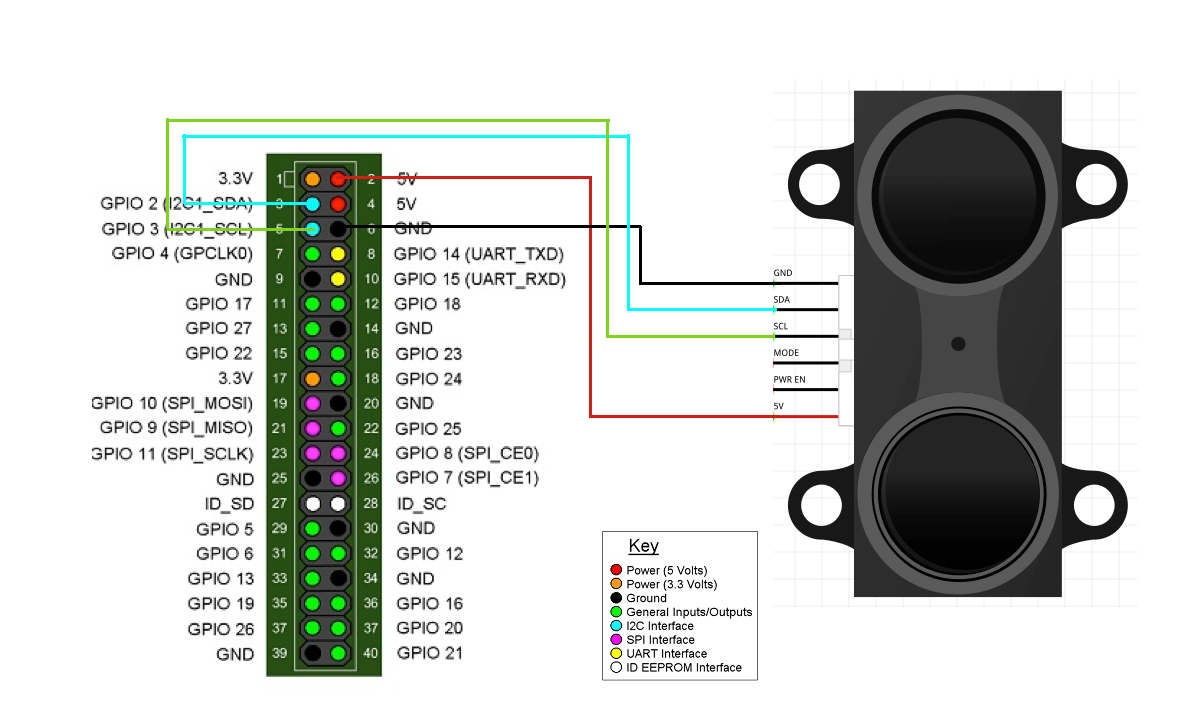
\includegraphics[scale=.4]{images/laderraspberryconnection.png}
	\caption{The pinout and wiring of the LIDAR and Raspberry Pi}
	\label{fig:wiringlidarpi}
\end{figure}

\begin{table}[H]
	\centering
	\begin{tabular}{|l|l|l|}
		\hline
		\textbf{Raspberry pin} & \textbf{Description} & \textbf{LIDAR pin} \\ \hline
		2 & 5V & Red \\ \hline
		5 & GND & Black \\ \hline
		4 & SCL & Green \\ \hline
		3 & SDA & Blue \\ \hline
	\end{tabular}
	\caption{Raspberry pins mapped to the LIDAR pins}
\end{table}

We started using a library called lidarLite, which provides a simple C interface to the LIDAR on a Raspberry. It is based on the WiringPi interface, which is a GPIO access library written in C for the BCM2835 SoC used in the Raspberry Pi. It is usable from C and C++ and many other languages with suitable wrappers. It was designed very familiarly to Arduino's wiring library.

With the lidarLite library, we managed to set up a connection using the I2C protocol. By enabling the built in I2C support in the Raspberry Pi kernel, and after the wiring of the components, a connection has been set up between the LIDAR laser and the controller.

%https://learn.adafruit.com/adafruits-raspberry-pi-lesson-4-gpio-setup/configuring-i2c
%https://github.com/answer17/lidarLite

A small program was written in order to test the output of the laser sensor, namely to read out the distance value of the next closes point in centimeters. 

% sample output here

This output is generated by the function called \textit{lidar\_read(int fd)} from the lidarLite library. This code simply calculates the low and high value from the sensor and returns the distance measurements in centimeters, in form of an integer value. The guide on how to compile and run this small test application is available in the Appendix \\ %TODO: Add readme.md from laser-module folder to appendix.

\lstinputlisting[firstline=47, lastline=64, title=lidarLite.c, language=C]{../code/laser-module/src/lidarLite.c}